\documentclass[10pt,a4paper]{article}
\usepackage{minted}
\usepackage[utf8]{inputenc}
\usepackage[spanish]{babel}
\parindent=0cm
\usepackage{amsmath}
\usepackage{amssymb,amsfonts,latexsym,cancel}
\usepackage{graphicx}
\usepackage{epstopdf}
\usepackage{dsfont}
\usepackage{float}
\usepackage{subfigure}
\usepackage{array}
\usepackage{longtable}
\newcolumntype{E}{>{$}c<{$}}
\setcounter{MaxMatrixCols}{40}
\usepackage{bm}
\usepackage{hyperref}
\hypersetup{
    colorlinks=true,
    linkcolor=blue,
    filecolor=magenta,      
    urlcolor=cyan,
}
\usepackage{forest}
%%%%%%%%%%%%%%%%%%%%%%%%%%%%%%%%%%%%
\usepackage[lmargin=1.5cm,rmargin=2cm,top=4cm,bottom=2.5cm,headheight=10pt,headsep=90pt]{geometry}

\usepackage{fancyhdr}
\usepackage{afterpage}
\pagestyle{fancy}
\fancyhf{}

\fancyhead{}%eliminar definicones previas
\fancyhead[C]{\textbf{UNIVERSIDAD DEL QUINDIO}\\[5pt]
	INGENIERÍA DE SISTEMAS Y COMPUTACIÓN\\[5pt] Analisis de Algoritmos\\[5pt]Contenido: Proyecto Final \\ Estudiantes: Jordy Diaz - Jennifer Suarez }
\title{Análisis Bibliométrico con Grafos}
\fancyhead[L]{\includegraphics[scale=0.5]{LogoUq.png}}

\renewcommand{\headrulewidth}{0pt}

\begin{document}

\maketitle
\thispagestyle{fancy} % Ensure the first page also has the fancy style

\begin{abstract}
El presente documento describe la metodología y implementación de los dos requerimientos correspondientes al Seguimiento 2 del proyecto final. El objetivo es realizar un análisis bibliométrico sobre una colección de artículos científicos utilizando técnicas de teoría de grafos. El primer requerimiento se centra en la construcción de una red de citaciones para analizar las relaciones de influencia entre artículos. El segundo requerimiento se enfoca en la identificación de clústeres temáticos mediante la creación de un grafo de co-ocurrencia de términos clave.
\end{abstract}

\tableofcontents
\newpage

\section{Requerimiento 1: Análisis de Red de Citaciones}
El script \texttt{requerimiento\_1\_grafos.py} tiene como finalidad construir y analizar una red de citaciones a partir de un archivo \texttt{.bib}. Esta red es un grafo dirigido donde los nodos son los artículos y las aristas representan las citas entre ellos. El análisis de esta red permite identificar artículos influyentes, la relación entre diferentes trabajos y la existencia de "escuelas de pensamiento".

\subsection{Metodología}
El proceso se divide en tres fases principales: carga de datos, construcción del grafo (explícito e inferido) y análisis de la estructura resultante.

\subsubsection{Fase 1: Carga de Datos}
Se utiliza la librería \texttt{bibtexparser} para leer y procesar el archivo \texttt{articulos\_con\_titulo\_y\_abstract.bib}. La función \texttt{cargar\_articulos} se encarga de esta tarea, devolviendo una lista de diccionarios donde cada diccionario representa un artículo con sus metadatos (ID, título, autor, año, etc.).

\subsubsection{Fase 2: Construcción del Grafo}
Esta es la fase central del script y se realiza en dos pasos dentro de la función \texttt{construir\_grafo\_citaciones}:

\begin{enumerate}
     \textbf{Adición de Citas Explícitas:} Se crea un grafo dirigido (\texttt{nx.DiGraph}). Se recorren todos los artículos y, si uno de ellos posee un campo \texttt{cites}, se interpreta su contenido para crear aristas directas desde el artículo actual hacia los artículos que cita. Estas aristas representan una relación de citación directa y verificada.
    
     \textbf{Inferencia de Citas por Similitud de Texto:} Dado que no todos los artículos tienen información de citas, se implementa un método para inferir relaciones. Se combinan el título y el abstract de cada artículo para crear un documento de texto representativo. Usando \texttt{TfidfVectorizer} de Scikit-learn, estos textos se convierten en vectores numéricos. Posteriormente, se calcula la similitud del coseno entre todos los pares de artículos. Si la similitud entre dos artículos supera un umbral y no existe una cita explícita, se infiere una arista del artículo más reciente al más antiguo, asumiendo que el trabajo más nuevo se basó en el más antiguo. La similitud calculada se almacena como el \textbf{peso} de la arista.
\end{enumerate}

\begin{minted}{python}
# Fragmento de la construcción del grafo
def construir_grafo_citaciones(articulos, inferir_por_similitud=True, top_n_similares=3):
    G = nx.DiGraph()
    articulos_por_id = {art.get('ID'): art for art in articulos if 'ID' in art}

    # --- PASO 1: Citas explícitas ---
    for articulo in articulos:
        # ... (código para añadir nodos y aristas explícitas)

    # --- PASO 2: Inferir citaciones por similitud ---
    if inferir_por_similitud and len(articulos) > 1:
        ids = [art.get('ID', art.get('title', 'N/A')[:30]) for art in articulos]
        years = [int(art.get('year', '0')) for art in articulos]
        textos = [art.get('title', '') + ' ' + art.get('abstract', '') for art in articulos]

        vectorizer = TfidfVectorizer(stop_words='english', min_df=2)
        tfidf_matrix = vectorizer.fit_transform(textos)
        matriz_similitud = cosine_similarity(tfidf_matrix)
        # ... (lógica para añadir aristas inferidas basadas en similitud y año)
    return G
\end{minted}

\subsubsection{Fase 3: Análisis del Grafo}
Una vez construido el grafo, se implementan dos funciones de análisis:
\begin{itemize}
     \texttt{encontrar\_camino\_minimo}: Utiliza el algoritmo de Dijkstra de \texttt{networkx} para encontrar la ruta de mayor influencia (no la más corta) entre dos nodos. Esto se logra definiendo el peso de cada arista como \texttt{1 - similitud}, de modo que el algoritmo prioriza las aristas con mayor similitud.
     \texttt{encontrar\_componentes\_fuertemente\_conexas}: Identifica subgrupos de artículos que están densamente interconectados, es decir, donde cada artículo del subgrupo puede ser alcanzado desde cualquier otro. Estos componentes representan "comunidades de investigación" o sub-campos temáticos muy cohesionados.
\end{itemize}

\subsubsection{Fase 4: Visualización del Grafo}
La visualización del grafo es un paso crucial para la interpretación de los resultados. La imagen generada permite una comprensión intuitiva de la estructura de la red de citaciones.

\begin{figure}[H]
    \centering
    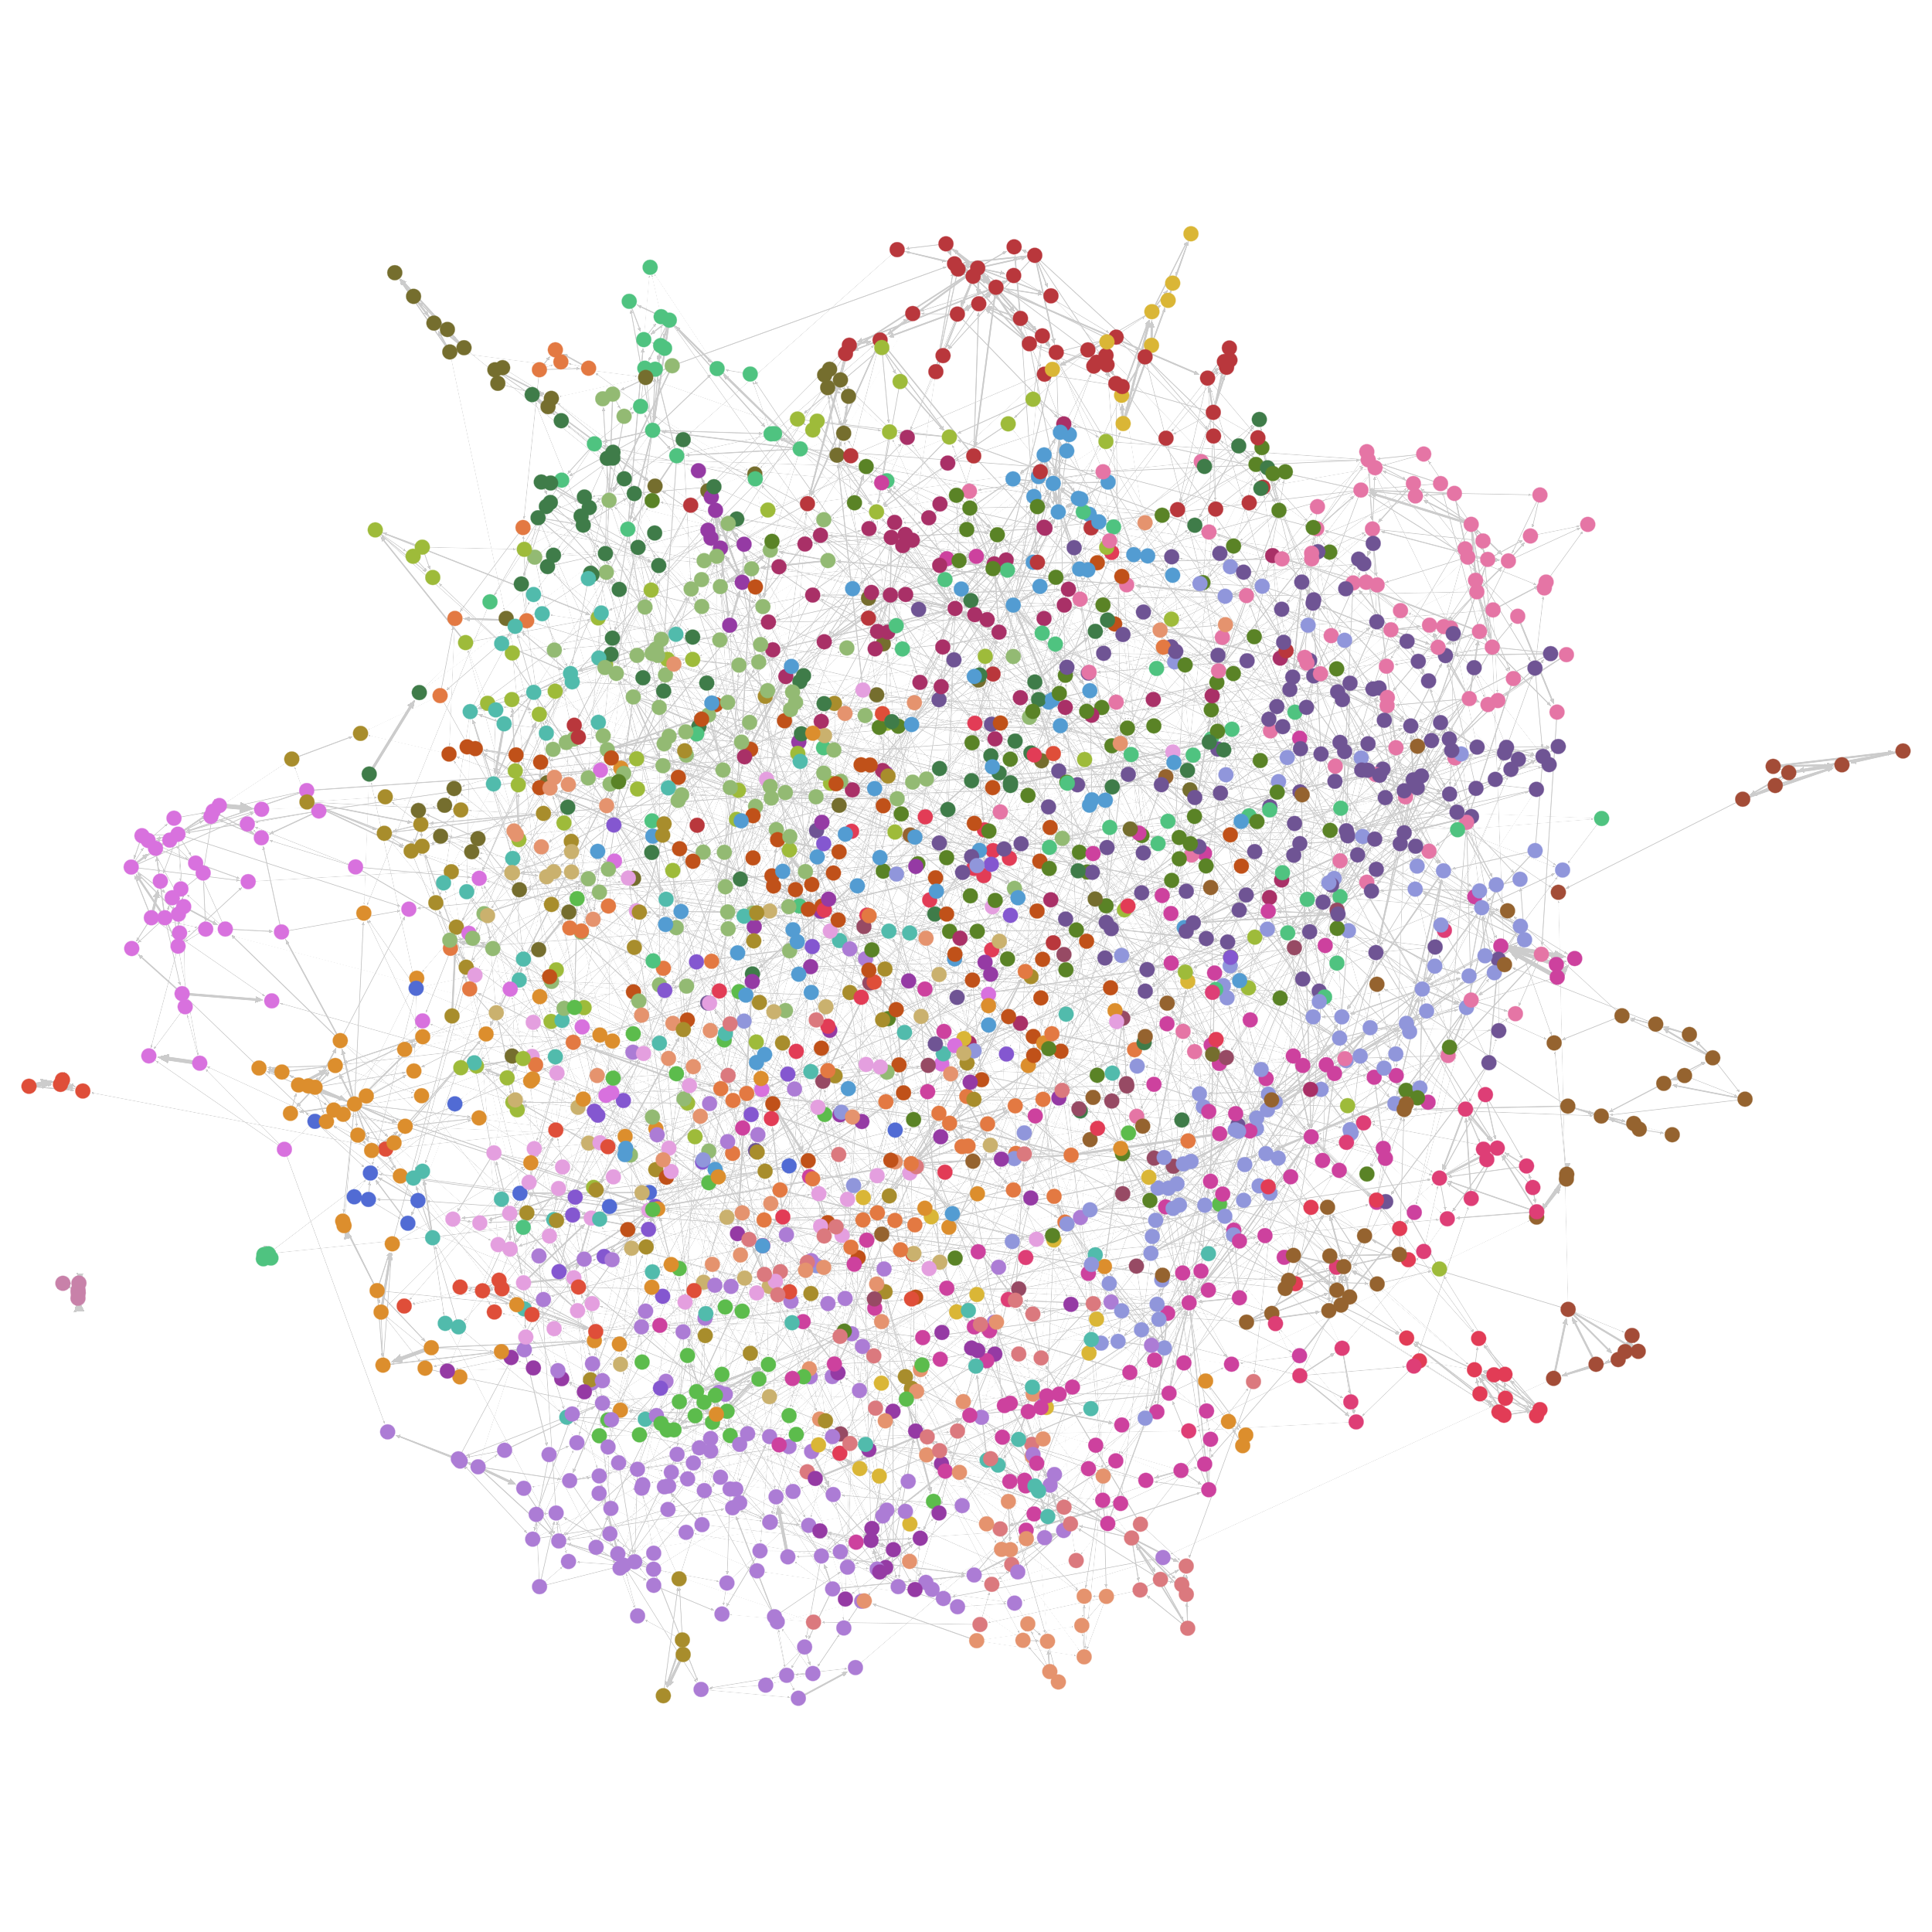
\includegraphics[width=0.9\textwidth]{GrafoCita.png}
    \caption{Visualización del Grafo de Citaciones.}
    \label{fig:grafo_cita}
\end{figure}

La Figura \ref{fig:grafo_cita} muestra la red de citaciones completa. En esta visualización:
\begin{itemize}
    \item Cada \textbf{nodo} representa un artículo científico de la colección.
    \item Las \textbf{aristas} (flechas) representan una cita, apuntando desde el artículo que cita hacia el artículo citado. Estas pueden ser explícitas o inferidas.
    \item La disposición espacial, generalmente controlada por un algoritmo de layout basado en fuerzas (como ForceAtlas2), agrupa los nodos de manera que los artículos con más conexiones entre sí aparecen más cerca.
    \item Los nodos con un alto grado de entrada (muchas flechas apuntando hacia ellos) pueden ser considerados trabajos seminales o muy influyentes. Los nodos con un alto grado de salida pueden ser artículos de revisión (reviews) o trabajos que sintetizan múltiples áreas.
\end{itemize}

\newpage
\section{Requerimiento 2: Análisis de Co-ocurrencia de Términos}
El script \texttt{requerimiento\_2\_grafos.py} busca descubrir los principales temas de investigación en la colección de artículos. Para ello, construye un grafo no dirigido donde los nodos son términos clave y las aristas indican que dos términos aparecen juntos frecuentemente en los mismos abstracts.

\subsection{Metodología}
El proceso consta de tres fases: extracción de los términos más relevantes, construcción del grafo de co-ocurrencia y, finalmente, filtrado y análisis para la identificación de temas.

\subsubsection{Fase 1: Extracción de Términos Relevantes}
Analizar la co-ocurrencia de todas las palabras de todos los abstracts sería computacionalmente costoso y generaría mucho ruido. Por ello, el primer paso es identificar un conjunto limitado de los términos más significativos. La función \texttt{extraer\_terminos\_relevantes} realiza esta tarea utilizando TF-IDF:
\begin{enumerate}
     Se vectorizan todos los abstracts usando \texttt{TfidfVectorizer}, configurado para considerar tanto palabras individuales como bigramas (pares de palabras, ej. "machine learning").
     A diferencia del Requerimiento 1, aquí no se comparan documentos entre sí. En su lugar, se suman los puntajes TF-IDF de cada término a lo largo de todo el corpus.
     Los 50 términos con el puntaje total más alto son seleccionados como los "términos clave" para el análisis.
\end{enumerate}

\subsubsection{Fase 2: Construcción del Grafo de Co-ocurrencia}
Con la lista de términos clave, la función \texttt{construir\_grafo\_coocurrencia} crea la red temática:
\begin{itemize}
     Se inicializa un grafo no dirigido (\texttt{nx.Graph}) y se añaden los términos clave como nodos.
     Se itera sobre cada abstract de la colección.
     Para cada abstract, se identifica cuáles de los términos clave aparecen en él.
     Se generan todas las combinaciones de pares de los términos encontrados. Para cada par, se crea una arista entre ellos o, si ya existe, se incrementa su atributo \texttt{weight}. El peso de la arista termina representando la frecuencia con la que dos términos clave aparecen juntos, indicando una fuerte relación temática.
\end{itemize}

\begin{minted}{python}
# Fragmento de la construcción del grafo de co-ocurrencia
def construir_grafo_coocurrencia(terminos, abstracts):
    G = nx.Graph()
    for termino in terminos:
        G.add_node(termino)

    for abstract in abstracts:
        terminos_en_abstract = []
        for termino in terminos:
            if re.search(r'\b' + re.escape(termino) + r'\b', abstract, re.IGNORECASE):
                terminos_en_abstract.append(termino)
        
        # Anadir una arista por cada par de terminos que co-ocuren
        for term1, term2 in itertools.combinations(terminos_en_abstract, 2):
            if G.has_edge(term1, term2):
                G[term1][term2]['weight'] += 1
            else:
                G.add_edge(term1, term2, weight=1)
    return G
\end{minted}

\subsubsection{Fase 3: Filtrado y Análisis del Grafo}
El grafo resultante puede ser muy denso. Para facilitar su interpretación, se realiza un post-procesamiento:
\begin{enumerate}
     \textbf{Filtrado:} Se eliminan las aristas cuyo peso es inferior a un umbral (ej. 5), conservando únicamente las relaciones temáticas más fuertes. Los nodos que quedan aislados tras este proceso son también eliminados.
     \textbf{Análisis:} Se calculan dos métricas principales:
    \begin{itemize}
         \textbf{Centralidad de Grado:} Se mide el grado de cada nodo (número de conexiones). Los nodos con mayor grado son los términos más centrales e importantes dentro del campo de estudio.
         \textbf{Componentes Conexas:} Se identifican los subgrupos de nodos que están conectados entre sí pero desconectados de otros subgrupos. Cada componente conexa representa un "clúster temático" o un área de investigación específica.
\end{itemize}
    \end{itemize}
\end{enumerate}

\subsubsection{Fase 4: Visualización del Grafo}
La visualización de la red de co-ocurrencia es fundamental para la interpretación de los clústeres temáticos identificados.

\begin{figure}[H]
    \centering
    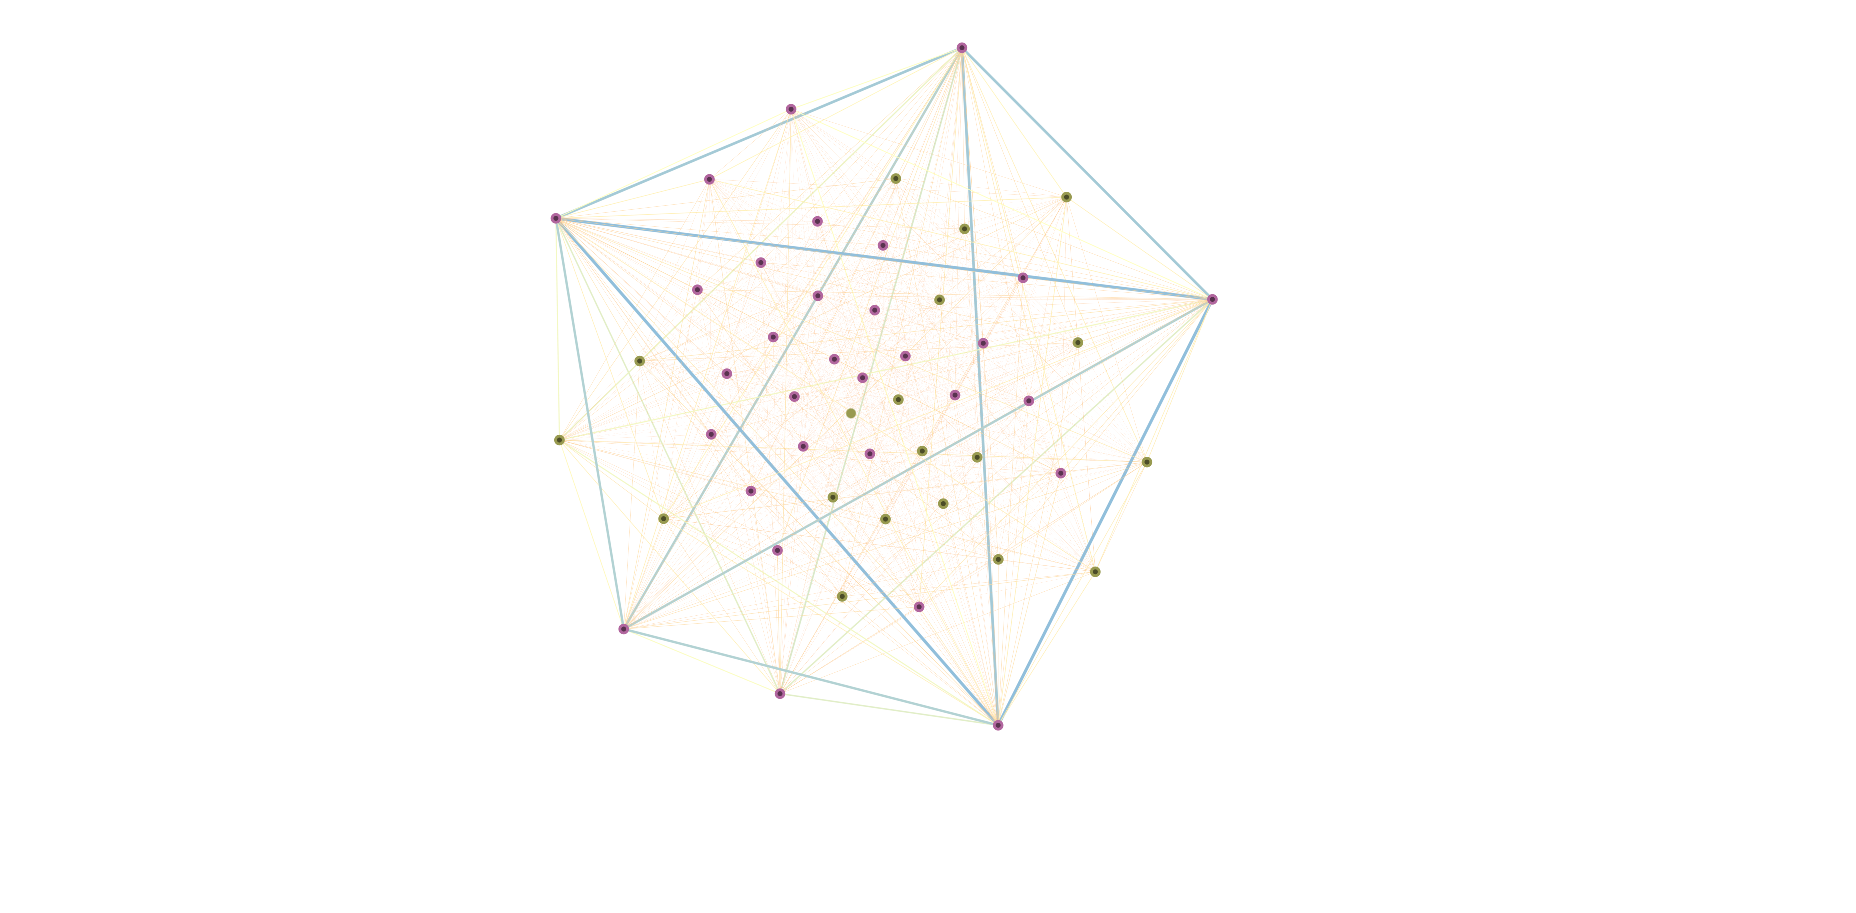
\includegraphics[width=0.9\textwidth]{GrafoCoocurrencia.png}
    \caption{Visualización del Grafo de Co-ocurrencia de Términos.}
    \label{fig:grafo_coocurrencia}
\end{figure}

La Figura \ref{fig:grafo_coocurrencia} presenta el grafo de co-ocurrencia de términos. En esta red:
\begin{itemize}
    \item Cada \textbf{nodo} es un término clave extraído del corpus de abstracts.
    \item Una \textbf{arista} entre dos nodos significa que ambos términos aparecen juntos con frecuencia en los mismos abstracts. El grosor de la arista puede ser proporcional a dicha frecuencia (peso), indicando una relación temática más fuerte.
    \item El \textbf{tamaño de la etiqueta} de un nodo puede ser proporcional a su centralidad de grado, destacando los conceptos más importantes y transversales del campo de estudio.
    \item Los \textbf{clústeres de nodos} densamente conectados, que se aprecian como "islas" en el grafo, corresponden a los grupos temáticos identificados por el algoritmo de componentes conexas. Estos representan las principales áreas de investigación o sub-temas en la colección de artículos.
\end{itemize}

\end{document}
